\documentclass{bioinfo}
\copyrightyear{2013}
\pubyear{2013}

\begin{document}
\firstpage{1}

\title[libRoadRunner]{libRoadRunner: A Universal, High Performance SBML Compliant Simulator}
\author[Sample \textit{et~al}]{A. Somogyi\,$^{1,*}$, M. T. Karlsson\,$^{2}$, M. Swat\,$^{1}$ and H. M Sauro\,$^3$\footnote{to whom correspondence should be addressed}}
\address{$^{1,3}$Biocomplexity Institute, Indiana University, Simon Hall MSB1, 212 S. Hawthorne Drive, Bloomington, IN  47405-7003
\\
$^{2}$Dune Scientific, 10522 Lake City Way NE, \#302 Seattle WA \\
$^{3}$Department of Bioengineering, University of Washington, Seattle, WA, 98195}

\history{Version 0.75}

\editor{Associate Editor: XXXXX}

\maketitle

\begin{abstract}

\section{Summary:}
Here we describe libRoadRunner, cross-platform, open-source,  high performance SBML compliant simulator written in C/C++. The primary motivation for developing libRoadRunner was to address deficiencies of existing simulators, in terms of speed of run, ease of use and ability to be used as a component in third-party applications. Additionally we focused on providing an extensible architecture with a wide variety of extension modules (such as...) that should address needs of biomodeling community. By creating an LLVM backend of a SBML model at runtime we achieved significant performance improvements over existing tools and enables to run very complex and elaborate biochemical models within very reasonable runtimes. To achieve full SBML compliance we implemeneted robust support for event handling and provided convenience fuunctions such as conservation analysis. We have also developed C and Python API which greatly facilitate reuse of libRoadRunner as a plugable component 


\section{Availability and Implementation:}
The core of libRoadRunner is written in C++ but to support linking with legacy C-code we developedn additional thin layer that supports a pure C API. To enable reuse of libRoadRunner in  scripting languages we provide extensive bindings for Python. libRoadRunner supports SBML via libSBML and uses CVODE for differential equation implementation and event handling. We also use NLEQ2 for solving nonlinear equations and LAPACK for stoichiometric analysis. We tested our library on Windows, Mac OS X and Linux and we provide binary packages for these operating systems. The library is open source and licensed under the Apache License, Version 2.0.

\section{Contact:} \href{hsauro@u.washington.edu}{hsauro@u.washington.edu}

\section{Supplementary information:}
Online documentation, build instructions and source code are available at http://www.libroadrunner.org

\end{abstract}

\section{Introduction}

There has been a long history~\citep{Bag01} of researchers developing biochemical network simulators. Most are monolithic making it very difficult to reuse the code for other applications. Recently there has been more interest in development reusable libraries. Most notable of these are COPASI, libSBMLSim, roadRunner, SOSLib and the Systems Biology Simulation Core Library (SBSCL). Each has strengths and weakness, for example COPASI has excellent support for optimization but its API can be challenging to use (see https://code.google.com/p/copasi-simple-api/), libSBMLSim passes all the tests in the SBML test suite but its API and functionality is somewhat limited, roadRunner is written in C\# which is excellent for .NET developers but less so for others, SOSLib is no longer supported but it has a reasonable API but does not support conservation analysis and finally SBSCL is written in Java which makes it an excellent choice for Java developers but less so for others and also doesn't support conservation analysis. All the libraries have performance issues and stability concerns (see benchmarking), most have problems tracking events except perhaps roadRunner and all have a non-extensible architectures.

Here we describe libRoadRunner which is based on previously developed C\# roadRunner [ref]. libRoadRunner is written in C++ with an additional C and Python API's. The C API was designed with the modeler in mind and offers a wide range of functionality and specific methods for rapid access to the core to improve performance in realtime interactive environments. libRoadRunner supports a plugin extension mechanism making it possible to easily write extensions to the core (See Plugins). One of the key and novel features of libRoadRunner is use of the LLVM (formerly Low Level Virtual Machine) which is designed for real-time optimization and dynamic compilation of application software. This has allowed us to develop the fastest biochemical simulator currently available. This is particularly important for large simulation applications e.g. multi-cell models where each cell runs several biochemical networks submodels. Figure~\ref{fig:01} shows the architectural overview of libRoadRunner.

\begin{figure}[!htpb]%figure2
\centerline{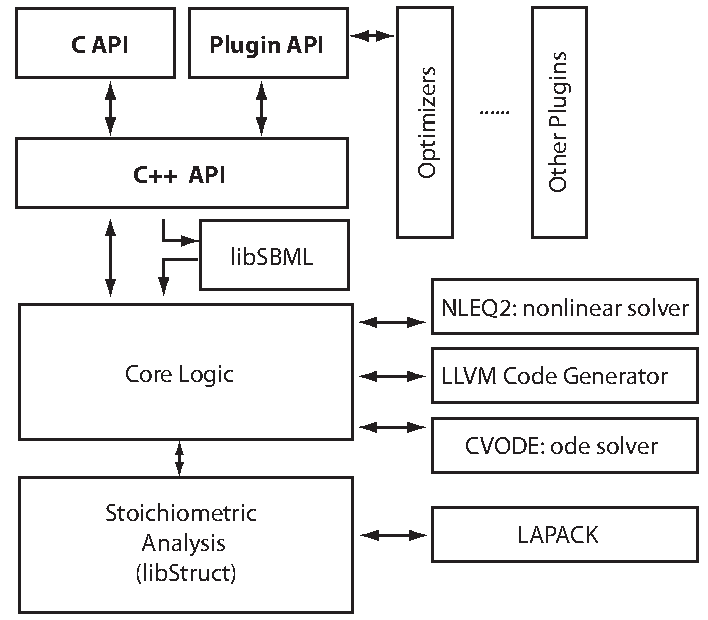
\includegraphics[scale=0.55]{roadRunnerOverview.pdf}}
\caption{Architectural Overview of libRoadRunner.}\label{fig:01}
\end{figure}

\begin{methods}
\section{Methods}

\subsection{Features}

List of features here

\subsection{LLVM Backend}

LLVM is a technology that allows dynamic compilation of code at runtime. This allows us to cast SBML models directly into native machine code at runtime. LLVM can generate runtime code for a large number of architectures, including on ARM (for example the  Raspberry Pi) but also for GPUs. In addition to GPU and CPU generated code the backend can be easily configured for other outputs. For example one option included with roadRunner is the ability to direct code generate to pure C code. Similarly simulation libraries can also be reconfigured such that a stochastic simulator would be incorporated. Because the configuration of the libRoadRunner LLVM-backend takes place in the RAM we avoid  the hassle of converting SBML to C, compiling on-the-fly and loading dynamic libararies. Consequently, we do not generate any temporary files. 

\subsection{Extensibility}

Extensibility was an importance consideration in the design of the roadRunner library as noted in the previous section. The easiest way to to add external new extensions by writing Python scripts, this is simple but may have the disadvantage of potentially poorer performance. The alternative is to write native code (C,C++, Fortran) plugins that can be loaded on demand by the roadRunner core. A plugin API is available as a pure C API so that plugins can be written in almost any language. Under Windows, a plugin is just a standard DLL. Plugins have full access to the roadRunner API which includes the ability to create new roadRunner instances. A primary advantage of plugins is that additional functionality can be developed without disturbing any of core roadRunner code. In addition, the plugin exposes a set of methods to allow generic access to any exported plugin functionality. This means that scripting languages such as Python can easily access a plugin without having to implement a new API for every plugin. Plugins also support a degree of runtime type information that allows graphical user interface applications to create user interfaces at runtime when the plugin is loaded. The roadRunner distribution comes with two plugins that illustrate how plugins can be built, these include a a plugin that implements the Levenberg-Marquardt algorithm (ref) that allows models to be fitted to experimental data and a smaller plugin that can be used to generate synthetic experimental data for testing the Levenberg-Marquardt plugin.


\subsection{Python API}

Two Python APIs were developed, a ctypes based library and customized SWIG binding. The SWIG binding is more comprehensive and Pythonic in its design and is the recommended for most external applications. It permits instantiations of multiple RoadRunner simulators and thus offers very natural way of using libRoadRunner as the Reaction-Kinetics engine in multi cell simulators such as CompuCell3D (www.compucell3d.org). The SWIG-based libRoadRunner Python API exposes most of the function of the actual simulator object that the end user needs to construct sophisticated SBML-based models.

ANDY - put more text about dictionaries, Pythonism of the API etc... 

The ctypes Python interface is used to specifically test the C API. 

\subsection{Performance}

We compared three other simulator libraries with libRoadRunner (ref), these included libSBMLSim (ref), COPASI (ref) and Systems Biology Simulation Core Library (ref). We tested the ability pass the SBML test suite, the ability to simulate very large models and the ability to simulate systems with large numbers of events. Table~\ref{Tab:01} lists the times recorded from the four different libraries based on three different types of model. The first model is a moderate sized model that tests the general performance in integration and evaluating the differential equations. The second model tests the ability of the libraries to scale to very large models and the third library tests the ability of the library to deal with large number of discrete events. The timings also include the amount of time requite to load the SBML model and compile it to executable code.
%
\begin{table}[!t]
\processtable{All times are in milliseconds. Test models are available at libroadrunner.org\label{Tab:01}}
{\begin{tabular}{llll}\toprule
Application & Simulation & Large Models & Event Handling\\\midrule
libRoadRunner & 23 & 45 & 67  \\
COPASI & 200 & 400 & fail\\
libSBMLSim & 450 & fail & fail\\
SBSCL & 500 & 800 & fail \\ \botrule
\end{tabular}}{}
\end{table}

\subsection*{Implementation Details}

The dedicated web site, libroadrunner.org includes all the necessary information concerning libRoadRunner including documentation for the C++ and C API, and documentation for the Python SWIG binding. Full build instructions are provided for Windows and Mac OS X. Build instructions for specific Linux disruptions can be obtained upon request particularly XYZ and ABC. All source code is stored on Github, documentation is generated via Doxygen and sphinc for Python. The build system is based around CMake, Linux binaries are generated using GCC, Mac binaries via CLang \citealp{Boffelli03} and Windows binaries via Visual Studio 2010. Binaries are provided for Windows, Mac OS X, including binaries for Python 2.7 on Windows and Mac OS X.


\subsection{Using libRoadRunner in multi-cell simulations}

As a proof of concept we have succesfully deployed libRoadRunner as Reaction-Kinetic solver engine in CompuCell3D. CompuCell3D is a simulation environment used to build multi-cell, single-cell based models of tissues. We have used Python API to associate with each CompuCell3D cell a collection of libRoadRunner-based simulators. Since CompuCell3D uses python scripting to describe its models integrating libRoadRunner was particularly easy. The clean design of the libRoadRunner Python API was helpful in designing intuitive part of the CompuCell3D Python API that deals with biochemical simulator handling. Previous versions of CompuCell3D relied on biochemical simulators that had either interpreted cores or used on-the-fly compilation and unlike libRoadRunner they were difficult to deploy and maintain. 

We ran Delta-Notch patterning simulation {\bf Swat03} on the array of 36 adjacent cells with different reaction-kinetics models solvers and determined that libRoadRunner solvers led to  2x shorter overall simulation runetimes as compared to the previous implementations present in older version of CompuCell3D. One should keep in mind that in multi-cell simulations time spend on solving reaction-kinetics models makes up only a fraction of the totoal runtime. Thus 2x  speedup of the overall simulation is quite significant and is representative of the high-performance focus of the new libRoadRunner. 
  

\end{methods}

\section{Discussion}

In this application note we describe a new high performance SBML compliant simulator. The reason for developing libRoadRunner was to satisfy a number of specific applications that require high performance, good SBML compatibility and broad functionality. These applications include interactive desktop simulation, multicellular simulations often requiring 10,000 or more of simultaneous simulations, and multi-session needs for web based interactive simulation.  For the future we are planning a number of additional features, these include new plugins, particularly alternative optimizers, and a bifurcation analysis plugin. Expand this: Currently used by: CompuCell3D, JDesigner, Tellurium, sysb.io

\section*{Acknowledgement}
We wish to acknowledge Frank Bergmann who together with Herbert Sauro wrote the original roadRunner library in C\#. In addition libStruct, the structural analysis library previously developed by Frank Bergmann and Ravi Rao. We wish to also thank Michal Galdzicki who assisted in putting together the libroadrunner.org website. Finally we wish to thank Stanley Gu for testing libRoadRunner in his web based environment.

\paragraph{Funding\textcolon} Work supported by the National Institute of General Medical Sciences of the National Institutes of Health under award numbers R01-GM081070. The content is solely the responsibility of the authors and does not necessarily represent the official views of the National Institutes of Health.

%\bibliographystyle{natbib}
%\bibliographystyle{achemnat}
%\bibliographystyle{plainnat}
%\bibliographystyle{abbrv}
%\bibliographystyle{bioinformatics}
%
%\bibliographystyle{plain}
%
%\bibliography{Document}


\begin{thebibliography}{}
\bibitem[Bofelli {\it et~al}., 2000]{Boffelli03} Bofelli,F., Name2, Name3 (2003) Article title, {\it Journal Name}, {\bf 199}, 133-154.

\bibitem[Bag {\it et~al}., 2001]{Bag01} Bag,M., Name2, Name3 (2001) Article title, {\it Journal Name}, {\bf 99}, 33-54.

\bibitem[Swat {\it et~al}., 2013]{Swat01} Swat,M.H., Thimas, G.L., Belmonte J.M., Shirinifard A, Hmeljak D, Glazier J.A (2013) Multi-Scale Modeling of Tissues Using CompuCell3D, {\it Methods Cell Biol.}, {\bf 110}, 325-366.

\bibitem[Yoo \textit{et~al}., 2003]{Yoo03}
Yoo,M.S. \textit{et~al}. (2003) Oxidative stress regulated genes
in nigral dopaminergic neurnol cell: correlation with the known
pathology in Parkinson's disease. \textit{Brain Res. Mol. Brain
Res.}, \textbf{110}(Suppl. 1), 76--84.

\bibitem[Lehmann, 1986]{Leh86}
Lehmann,E.L. (1986) Chapter title. \textit{Book Title}. Vol.~1, 2nd edn. Springer-Verlag, New York.

\bibitem[Crenshaw and Jones, 2003]{Cre03}
Crenshaw, B.,III, and Jones, W.B.,Jr (2003) The future of clinical
cancer management: one tumor, one chip. \textit{Bioinformatics},
doi:10.1093/bioinformatics/btn000.

\bibitem[Auhtor \textit{et~al}. (2000)]{Aut00}
Auhtor,A.B. \textit{et~al}. (2000) Chapter title. In Smith, A.C.
(ed.), \textit{Book Title}, 2nd edn. Publisher, Location, Vol. 1, pp.
???--???.

\bibitem[Bardet, 1920]{Bar20}
Bardet, G. (1920) Sur un syndrome d'obesite infantile avec
polydactylie et retinite pigmentaire (contribution a l'etude des
formes cliniques de l'obesite hypophysaire). PhD Thesis, name of
institution, Paris, France.

\end{thebibliography}
\end{document}
